% Generated by book/tools/notebook_to_tex.py. Do not edit by hand.

\chapter[작은 BERT 사전학습 (English MLM)]{작은 BERT 사전학습 (English MLM Pretraining)}

\label{ch:20}

\markboth{작은 BERT 사전학습 (English MLM)}{작은 BERT 사전학습 (English MLM)}

\chaptermeta{20_en_bert_pretrain/20_en_bert_pretrain.ipynb}{https://colab.research.google.com/github/yoon-gu/neuqes-101/blob/master/20_en_bert_pretrain/20_en_bert_pretrain.ipynb}{영어 일반 도메인 위키 코퍼스로 작은 BERT를 MLM 방식으로 직접 사전학습}



\index{1BERT pretraining@BERT pretraining}

\index{1Masked Language Modeling@Masked Language Modeling}

\index{1MLM@MLM}

\index{1BertConfig@BertConfig}

\index{1BertForMaskedLM@BertForMaskedLM}

\index{1DataCollatorForLanguageModeling@DataCollatorForLanguageModeling}

\index{1group texts@group\_texts}

\index{1perplexity@perplexity}

\index{1random initialization@random initialization}

\index{1Wikitext 103@Wikitext-103}

\index{1bert base uncased@bert-base-uncased}

\index{0작은 BERT@작은 BERT}

\index{0사전학습@사전학습}

\index{0마스크드 언어 모델링@마스크드 언어 모델링}

\index{0마스크 토큰@마스크 토큰}

\index{0퍼플렉서티@퍼플렉서티}

\index{0일반 도메인@일반 도메인}

\index{0사전학습량 곡선@사전학습량 곡선}

\index{1perplexity curve@perplexity curve}

\index{1scaling curve@scaling curve}

\index{1epoch saturation@epoch saturation}

\index{0데이터 병목@데이터 병목}

\index{1AutoTokenizer@AutoTokenizer}

\index{1AutoModelForMaskedLM@AutoModelForMaskedLM}

\index{1Trainer@Trainer}

\index{1TrainingArguments@TrainingArguments}

\index{1mlm probability@mlm\_probability}

\index{1ignore index@ignore\_index}

\index{1labels 100@labels=-100}

\index{1mask token prediction@mask token prediction}

\index{1top k prediction@top-k prediction}

\index{1save pretrained@save\_pretrained}

\index{1Salesforce wikitext@Salesforce/wikitext}

\index{1random baseline@random baseline}

\index{1language modeling head@language modeling head}

\index{0언어 모델링 헤드@언어 모델링 헤드}

\index{0마스킹 비율@마스킹 비율}

\index{080 10 10 규칙@80/10/10 규칙}

\index{0무작위 초기화@무작위 초기화}

\index{0체크포인트 저장@체크포인트 저장}

\index{0위키텍스트@위키텍스트}



\section{변화추적표}

\begin{booktable}{20장 변화추적표}{tab:ch20-01}
\begin{adjustbox}{max width=\textwidth}
\begin{tabular}{@{}lllllll@{}}
\toprule
Ch & 모델 & 토크나이저 & 데이터 & Output Head & Activation & Loss \\
\midrule

17 & klue/bert-base & WordPiece (한국어, 사전학습) & KLUE-YNAT 합성 multi-label & \inlinecode{Linear(H,\ 7)} & sigmoid (각각) & \inlinecode{BCEWithLogitsLoss} \\
18 & klue/bert-base + 보조 & WordPiece (한국어, 사전학습) & KLUE-YNAT 합성 + 보조 라벨 & 메인(7) + 보조 & sigmoid + 태스크별 & \inlinecode{BCEWithLogitsLoss\ +\ λ·L\_aux} \\
19 & --- (토크나이저 학습 전용) & WordPiece + WordLevel (둘 다 직접 학습) & Yelp text + NSMC text & --- & --- & --- \\
\textbf{20 \(\leftarrow\) 여기} & \textbf{작은 BERT (직접, scratch)} & \textbf{\inlinecode{bert-base-uncased} 토크나이저 (가져옴)} & \textbf{Wikitext-103 paragraphs (일반 도메인)} & \textbf{MLM head} & softmax (MLM) & \textbf{\inlinecode{CrossEntropyLoss} (masked token)} \\
21 (다음) & \ref{ch:20}장 사전학습 BERT + 분류 헤드 & (\ref{ch:20}장과 동일) & Yelp 이진화 (다른 도메인 transfer) & \inlinecode{Linear(H,\ 2)} & softmax & \inlinecode{CrossEntropyLoss} \\
\bottomrule
\end{tabular}
\end{adjustbox}
\end{booktable}

전체 장 표는 \href{https://github.com/yoon-gu/neuqes-101\#챕터별-변화추적표}{루트 README.md}를 참고하세요.

\textbf{Phase 3 안에서의 위치} --- \ref{ch:19}장 (토크나이저 학습) \(\to\) \ref{ch:20}장 (모델 사전학습) \(\to\) \ref{ch:21}장 (분류 fine-tune). 사전학습 모델을 \emph{받아서 fine-tune} 하던 Phase 1·2 의 흐름을 이번엔 \emph{직접 만들어} 봅니다.



\section{변경점: \ref{ch:19}장 대비}

\begin{booktable}{20장 변경점 요약}{tab:ch20-02}
\begin{adjustbox}{max width=\textwidth}
\begin{tabular}{@{}lll@{}}
\toprule
축 & \ref{ch:19}장 (토크나이저 학습 전용) & \ref{ch:20}장 (작은 BERT scratch MLM) \\
\midrule

\textbf{이 장의 task} & 토크나이저 학습 (모델 없음) & \textbf{모델 사전학습 (MLM)} \(\leftarrow\) \emph{유일한 변화} \\
모델 & 없음 & \textbf{작은 \inlinecode{BertForMaskedLM} (random init, 약 11M params)} \\
토크나이저 & WordPiece + WordLevel \emph{직접 학습} & \textbf{\inlinecode{bert-base-uncased} \emph{가져옴}} (vocab 30,522) \\
데이터 & Yelp text + NSMC text (vocab 학습용) & \textbf{Wikitext-103 paragraphs (일반 도메인 MLM 학습용)} \\
Loss & 없음 (vocab + merge rules 가 산출물) & \textbf{\inlinecode{CrossEntropyLoss} (masked token 위치만)} \\
산출물 & tokenizer json 파일 4 종 & \textbf{모델 체크포인트} (\inlinecode{./ch20\_small\_bert\_mlm}) --- \ref{ch:21}장 재사용 \\
\bottomrule
\end{tabular}
\end{adjustbox}
\end{booktable}

\begin{quote}
\textbf{변경점 한 가지 원칙} --- Phase 3 안에서 \emph{모델 축} 이 변합니다 (없음 \(\to\) 작은 BERT scratch). 토크나이저는 \emph{직접 학습이 가능함을 본 뒤} 표준으로 돌아옵니다 --- \inlinecode{bert-base-uncased} 가 \emph{공개되어 검증된} vocab 이라 사전학습 안정성이 높음. 토크나이저 \emph{학습 절차} 와 \emph{모델 학습 절차} 가 두 장으로 분리되어 각각의 메커니즘이 또렷이 보이게 합니다.
\end{quote}

\subsection{왜 모델만 직접 학습하는가}

(1) \textbf{vocab 신뢰성} --- \ref{ch:19}장의 vocab 8K 토크나이저는 5K 문장 학습이라 어휘 커버리지가 좁음. \inlinecode{bert-base-uncased} 의 30,522 vocab 은 Wikipedia + BookCorpus 로 학습되어 \emph{영어 일반 분포} 를 잘 표현. 모델 학습이 vocab 노이즈에 영향받지 않음. (2) \textbf{다음 장 호환} --- \ref{ch:21}장에서 같은 토크나이저로 분류 fine-tune 하면, \emph{문체가 다른} downstream 입력에도 안정. (3) \textbf{표준 패턴} --- 실무에서도 보통 \emph{모델은 직접 사전학습하지만 vocab 은 검증된 것} 을 쓰는 패턴 (예: HF \inlinecode{roberta-base} 도 GPT-2 의 BPE 그대로 가져옴).

\subsection{왜 일반 위키로 사전학습하는가}

원본 BERT (Devlin et al., 2018) 는 \emph{영어 Wikipedia + BookCorpus} 라는 \textbf{일반 도메인} 코퍼스로 사전학습한 뒤, \emph{완전히 다른 downstream task} (GLUE, SQuAD 등) 로 fine-tune 했습니다. 본 장도 같은 패턴 --- Wikitext-103 \emph{일반 위키 paragraphs} 로 MLM 사전학습 \(\to\) \ref{ch:21}장에서 \emph{Yelp 리뷰(식당·업체)} 라는 \emph{다른 도메인} 으로 transfer.

만약 Yelp text 로 MLM 사전학습한 뒤 Yelp 분류로 fine-tune 하면 \emph{domain-adaptive pretraining} (DAPT) 에 가까워져 \emph{일반 표상 학습 \(\to\) 다른 task transfer} 의 본질이 흐려집니다. \emph{일반 도메인 \(\to\) 다른 도메인 transfer} 가 \emph{진짜 사전학습-fine-tune 패러다임}. \ref{ch:22}장 (한국어 위키 \(\to\) NSMC 분류) 가 같은 패턴.



\section{손실 함수의 변화: MLM}

이전 분류 장들 (\ref{ch:11}--\ref{ch:18}장) 의 loss 는 \emph{문장 한 개에 라벨 하나}. 이 장은 \emph{문장 안의 가려진 토큰들} 을 맞춰야 합니다 --- 토큰 위치 하나하나가 \emph{분류 task} 가 됩니다.

\subsection{수식}

입력 토큰 시퀀스 \(x = (x_1, \dots, x_n)\) 의 일부를 무작위로 \texttt{{[}MASK{]}} 로 가린 뒤, 모델이 \emph{원래 토큰} 을 예측:

\begin{equation}
\label{eq:ch20-01}
L_{\text{MLM}} = -\frac{1}{\vert{}M\vert{}} \sum_{i \in M} \log P(x_i \mid x_{\setminus M})
\end{equation}

식~\eqref{eq:ch20-01}은 이 절에서 사용하는 핵심 관계를 정리한 것입니다.

\begin{itemize}
\tightlist
\item
  \(M\): 가려진 위치 집합 (전체 토큰의 15\%)
\item
  \(P(x_i \mid x_{\setminus M})\): 모델이 \(i\) 번 위치에 \emph{원래 토큰} 을 예측할 확률 (vocab 30,522 차원 softmax)
\item
  \(\vert{}M\vert{}\): 가려진 토큰 수로 평균
\end{itemize}

각 가려진 위치에서 \emph{vocab 전체에 대한 \inlinecode{CrossEntropyLoss}}. 분류 헤드의 K (이전 장들의 2, 5, 7) 가 이번엔 \textbf{V = 30,522} 로 폭증.

\subsection{수치 예시}

\begin{booktable}{20장 손실 수치 예시}{tab:ch20-03}
\begin{adjustbox}{max width=\textwidth}
\begin{tabular}{@{}lll@{}}
\toprule
모델 상태 & 정답 토큰 확률 & \(-\log p\) \\
\midrule

균등 추측 (random init 초기) & \(1/30522 \approx 3.28 \times 10^{-5}\) & \textbf{10.33} \(\leftarrow\) random baseline \\
unigram --- 빈도만 아는 단계 & 코퍼스 빈도 그대로 & \textbf{7.25} \(\leftarrow\) 이 장이 넘어서야 할 기준선 \\
\textbf{이 장 도달점} (5K paragraphs \(\times\) 2 epoch) & --- & \textbf{7.06 - 7.13} \(\leftarrow\) 실측 (train 7.07 / eval 7.06-7.13) \\
약하게 학습 (정답 확률 0.01) & \(0.01\) & 4.61 \\
잘 학습된 작은 BERT (정답 확률 0.05-0.1) & \(0.05\) - \(0.1\) & 2.3 - 3.0 (이 셋업의 사정거리 밖) \\
큰 사전학습 BERT (정답 확률 0.3+) & \(0.3\) & 1.20 \\
완벽 (정답 확률 1.0) & \(1.0\) & 0.00 \\
\bottomrule
\end{tabular}
\end{adjustbox}
\end{booktable}

\textbf{관전 포인트}:

\begin{itemize}
\tightlist
\item
  학습 첫 step 의 loss 가 약 10 부근이면 random init 직후 \emph{균등 추측} 상태. 첫 100 step 안에 빠르게 떨어지면 vocab 정상.
\item
  \textbf{이 장의 목표는 \inlinecode{unigram\ 기준선\ (7.25)} 을 넘어서는 데까지} 입니다. 실제로 2 epoch 뒤 train loss 약 7.07, eval loss 약 7.06-7.13 에 도달합니다 --- \emph{“어떤 토큰이 흔한가”} 를 막 새긴 단계. 표의 loss 는 train/eval 공통 척도이고, 이 장에선 두 값이 거의 붙어 있습니다. 모델 생성 직전에 \inlinecode{set\_seed(SEED)} 를 걸어 두었으므로, 직접 돌려도 위 값이 소수점 둘째 자리까지 그대로 재현됩니다.
\item
  \emph{vocab 의 일부 후보를 추려내는} 단계 (2.5-4.0) 는 \textbf{이 셋업으로는 도달하지 않습니다.} 부록 \inlinecode{20\_en\_bert\_pretrain\_scaling} 에서 16 epoch 까지 늘려도 loss 는 약 6.5 (ppl 697) 에서 평탄해집니다 --- 더 내리려면 epoch 이 아니라 \textbf{데이터} 를 늘려야 합니다 ( 변형 참조).
\item
  작은 모델 + 5K paragraphs + 2 epoch 으로 \emph{완벽} 은 불가능 --- 그러나 \ref{ch:21}장의 fine-tune 출발점으로는 충분.
\end{itemize}

\subsection{Perplexity}

언어 모델 표준 metric. \(\text{PPL} = e^{L}\) --- \emph{모델이 다음 토큰을 평균 몇 후보 중에서 고민하는가} 의 직관:

\begin{booktable}{20장 Perplexity 표}{tab:ch20-04}
\begin{adjustbox}{max width=\textwidth}
\begin{tabular}{@{}lll@{}}
\toprule
MLM loss & PPL & 해석 \\
\midrule

10.33 & 30,522 & 균등 (전체 vocab) \\
7.25 & 1,412 & unigram --- 빈도만 아는 단계 \\
\textbf{7.13} & \textbf{1,253} & \(\leftarrow\) \textbf{이 장 2 epoch 실측} \\
6.55 & 697 & 부록에서 16 epoch 까지 늘린 결과 \\
5.0 & 148 & vocab 의 일부로 좁혀짐 \\
3.0 & 20 & 20 개 후보 중에서 결정 \\
1.0 & 2.7 & 거의 결정적 \\
\bottomrule
\end{tabular}
\end{adjustbox}
\end{booktable}

\begin{quote}
이전 분류 장의 \inlinecode{random\ baseline\ =\ log\ K} (K=2 \(\to\) 0.69, K=7 \(\to\) 1.95) 와 같은 직관을 \emph{vocab 차원에 확장} 한 게 MLM. \inlinecode{ln(30522)\ ≈\ 10.33} 이 그 random baseline.
\end{quote}



\section{토크나이저 노트}

이 장부터 토크나이저는 \emph{표준 사전학습 모델 것} 을 가져옵니다.

\begin{itemize}
\tightlist
\item
  \inlinecode{AutoTokenizer.from\_pretrained("bert-base-uncased")} --- 영어 BERT 의 표준 WordPiece.
\item
  vocab\_size = 30,522 (\ref{ch:19}장의 8K 와 비교해 약 4 배).
\item
  학습 코퍼스 = Wikipedia (영어) + BookCorpus \(\to\) 영어 일반 분포가 잘 반영.
\item
  특수 토큰: \texttt{{[}PAD{]}=0}, \texttt{{[}UNK{]}=100}, \texttt{{[}CLS{]}=101}, \texttt{{[}SEP{]}=102}, \texttt{{[}MASK{]}=103}.
\end{itemize}

\subsection{같은 문장의 토큰화 --- \ref{ch:19}장 직접 학습 vs \ref{ch:20}장 가져옴}

\inlinecode{"The\ capital\ of\ France\ is\ Paris,\ located\ on\ the\ Seine\ river."} 같은 \emph{일반 위키풍} 문장이:

\begin{itemize}
\tightlist
\item
  \textbf{\ref{ch:19}장의 8K WordPiece (Yelp 5K 학습)}: 학습 코퍼스 (Yelp) 분포에 \emph{최적화} 되어 있어 \emph{위키 도메인 단어} (\inlinecode{Seine}, \inlinecode{capital}, \inlinecode{located} 등) 가 작은 조각으로 쪼개짐 --- Yelp 에 적게 등장하는 어휘일수록 더 잘게 분할.
\item
  \textbf{\ref{ch:20}장의 \inlinecode{bert-base-uncased} 30K WordPiece (Wiki + BookCorpus 학습)}: 위키 어휘를 \emph{덜 쪼개짐}. 30K vocab + 일반 영어 학습이라 일반 도메인 + Yelp 같은 task 도메인 \emph{둘 다} 폭넓게 커버.
\end{itemize}

본 장의 사전학습 데이터 (Wikitext-103) 와 토크나이저 (\inlinecode{bert-base-uncased}) 가 \emph{둘 다 일반 위키 분포} 라 \emph{vocab 미스매치} 가 작습니다. \ref{ch:21}장에서 Yelp 분류로 fine-tune 할 때도 같은 토크나이저로 \emph{문체 다른} 도메인을 처리 --- 일반 영어 어휘는 거의 덜 쪼개지고, \emph{Yelp 리뷰 특유 표현} 만 약간 더 분할되는 정도.

\subsection{토크나이저와 모델의 결합}

\ref{ch:19}장 §5-4 의 cross-language 실험에서 봤듯, \emph{학습 언어가 다른} 토크나이저를 모델에 끼우면 거의 100\% UNK 가 됩니다. 모델 weight 와 vocab 은 \emph{함께 학습되어} 그 vocab 의 토큰 임베딩 공간에서 의미를 형성합니다.

이 장에서 \emph{토크나이저는 vocab 만 빌려오고 모델은 random init} 입니다 --- 즉 \emph{vocab 구조} 와 \emph{토큰 임베딩 의미} 가 분리됩니다. 학습 초기에는 임베딩이 random 이라 vocab 구조의 가치가 안 보이지만, MLM 으로 학습이 진행되면 임베딩이 vocab 구조에 \emph{맞춰 정렬} 됩니다 --- \emph{이 장의 본질이 바로 그 정렬 과정}.

\begin{quote}
\ref{ch:21}장부터는 \emph{이 장의 모델 + 토크나이저 쌍} 을 통째로 가져가 fine-tune. 둘은 \emph{함께 가야} 의미가 유지됩니다.
\end{quote}



\section{환경 준비}

설치가 끝나면 \textbf{라이브러리 버전을 먼저 찍습니다.} 같은 \inlinecode{seed} 로 돌려도 \inlinecode{transformers}·\inlinecode{datasets} 가 올라가면 수치가 미세하게 달라질 수 있어서, 아래 출력이 이 장에 실린 값과 다르다면 \emph{버전 차이} 를 먼저 의심하면 됩니다.



\textbf{baseline VRAM} (CUDA 환경에서만 의미 있는 출력 --- Colab T4 기준):



\Needspace{5\baselineskip}
\begin{lstlisting}
!nvidia-smi
\end{lstlisting}



\section{\texorpdfstring{토크나이저 로드}{토크나이저 로드}}

vocab 30,522 의 영어 WordPiece. \emph{모델은 random init} 이지만 토크나이저는 \emph{완성품} 을 가져옵니다.



\Needspace{11\baselineskip}
\begin{lstlisting}
TOKENIZER_NAME = "bert-base-uncased"
tokenizer = AutoTokenizer.from_pretrained(TOKENIZER_NAME)

print(f"tokenizer:        {TOKENIZER_NAME}")
print(f"vocab_size:       {tokenizer.vocab_size:,}")
print(f"model_max_length: {tokenizer.model_max_length}")
print(f"special tokens:")
for name in ("pad_token", "unk_token", "cls_token", "sep_token", "mask_token"):
    tok = getattr(tokenizer, name)
    tid = tokenizer.convert_tokens_to_ids(tok) if tok is not None else None
    print(f"  {name:>11}: {tok!r:>10}  (id={tid})")

\end{lstlisting}

\noindent\emph{앞뒤 블록은 모두 텍스트를 모델 입력 텐서로 바꾸는 단계입니다. 길이를 나누어 같은 흐름을 단계별로 확인합니다.}

\Needspace{8\baselineskip}
\begin{lstlisting}[firstnumber=13]
SAMPLE = "The capital of France is Paris, located on the Seine river."
enc = tokenizer(SAMPLE, return_tensors="pt")
tokens = tokenizer.convert_ids_to_tokens(enc["input_ids"][0])
print(f"\nsample: {SAMPLE!r}")
print(f"tokens ({len(tokens)}): {tokens}")
print(f"ids:    {enc['input_ids'][0].tolist()}")
\end{lstlisting}

\begin{codeRead}
\textbf{1행}의 \inlinecode{TOKENIZER\_NAME = ...}에서는 이후 분석에서 사용할 값을 준비합니다. \textbf{2행}의 \inlinecode{tokenizer = ...}에서는 이후 분석에서 사용할 값을 준비합니다. \textbf{8행}의 \inlinecode{for name in ("pad\_token",...}에서는 앞 단계에서 만든 값을 바탕으로 다음 계산을 수행합니다.
\end{codeRead}

\noindent\textbf{출력.}
\begin{bookoutputbox}
tokenizer:        bert-base-uncased
vocab_size:       30,522
model_max_length: 512
special tokens:
    pad_token:    '[PAD]'  (id=0)
    unk_token:    '[UNK]'  (id=100)
    cls_token:    '[CLS]'  (id=101)
    sep_token:    '[SEP]'  (id=102)
   mask_token:   '[MASK]'  (id=103)

sample: 'The capital of France is Paris, located on the Seine river.'
tokens (15): ['[CLS]', 'the', 'capital', 'of', 'france', 'is', 'paris', ','...
ids: [101, 1996, 3007, 1997, 2605, 2003, 3000, 1010, 2284, 2006, 1996, 1647...
\end{bookoutputbox}
\par\vspace{0.9em}



\section{데이터 준비}

원본 BERT 가 영어 Wikipedia + BookCorpus 라는 \emph{일반 도메인} 코퍼스로 사전학습한 정신을 따라, 본 장도 \textbf{Wikitext-103} 본문으로 MLM 사전학습합니다 --- \emph{task 도메인 (Yelp 리뷰(식당·업체)) 으로 사전학습하면 domain-adaptive pretraining 에 가까워져 사전학습의 진짜 메시지 (일반 표상 학습 \(\to\) 다른 task 로 transfer) 가 흐려지기 때문}.

\textbf{원본}: \inlinecode{Salesforce/wikitext}, config \inlinecode{wikitext-103-raw-v1} (CC-BY-SA, 정제된 영문 위키 paragraphs). HF Hub 정제본 --- line 단위로 이미 정리되어 있어 빈 줄 / 너무 짧은 줄 / 너무 긴 줄만 제외하면 바로 사용 가능. \ref{ch:21}장의 분류 fine-tune (Yelp 이진) 은 \emph{완전히 다른 도메인} --- 사전학습 \(\to\) fine-tune transfer 메시지가 정직해집니다. \ref{ch:22}장의 한국어 (한국어 Wikipedia paragraphs) 와 \emph{대칭} 패턴.



\section{\texorpdfstring{토큰화와 토큰 그룹화}{토큰화 + group\_texts --- HF run\_mlm.py 표준 패턴}}

MLM 사전학습의 표준 입력 포맷은 \emph{고정 길이 블록}. 변동 길이 문장에 그대로 padding 하면 \emph{손실}: (a) 짧은 문장이 많으면 PAD 비율이 높아 GPU 시간 낭비, (b) 긴 문장은 truncation 으로 정보 손실.

\textbf{해결책}: 모든 문서를 \emph{이어 붙여 토큰 스트림} 으로 만든 뒤, \inlinecode{block\_size=128} 단위로 자름. 문장 경계가 사라지는 trade-off 가 있지만, BERT 사전학습은 \emph{임의 위치의 토큰 예측} 이라 문장 경계가 중요하지 않음.

Wikitext-103 paragraphs 는 \emph{제한 50-2000자 필터링} 으로 평균 문장 길이가 일정 (수백 자 위주). 5,000 paragraphs 가 \inlinecode{block\_size=128} 로 잘리면 약 5,352 블록 (약 68만 토큰) 으로 정리됩니다. 코드는 HF \inlinecode{examples/pytorch/language-modeling/run\_mlm.py} 의 \inlinecode{group\_texts} 함수를 그대로 따른 표준 패턴.



\Needspace{11\baselineskip}
\begin{lstlisting}
BLOCK_SIZE = 128

def tokenize_function(examples):

    return tokenizer(examples["text"], add_special_tokens=False, truncation=False)

tokenized_train = ds_train_raw.map(
    tokenize_function, batched=True, remove_columns=["text"],
)
tokenized_eval = ds_eval_raw.map(
    tokenize_function, batched=True, remove_columns=["text"],
)
print(f"tokenized_train: {tokenized_train}")
print(
    f"first 30 input_ids of sample 0: "
    f"{tokenized_train[0]['input_ids'][:30]}"
\end{lstlisting}

\noindent\emph{앞 블록은 텍스트를 모델 입력 텐서로 바꾸는 단계입니다. 이어지는 블록에서는 앞에서 만든 중간 값을 다음 계산으로 넘기는 단계로 넘어갑니다.}

\Needspace{5\baselineskip}
\begin{lstlisting}[firstnumber=17]
)
\end{lstlisting}

\noindent\textbf{출력.}
\begin{bookoutputbox}
tokenized_train: Dataset({
    features: ['input_ids', 'token_type_ids', 'attention_mask'],
    num_rows: 5000
})
first 30 input_ids of sample 0: [20222, 12131, 10131, 4819, 15272, 1010, 19...
\end{bookoutputbox}
\par\vspace{0.9em}



\Needspace{11\baselineskip}
\begin{lstlisting}
def group_texts(examples):
    '''HF 표준 group_texts — 모든 토큰 스트림을 이어 붙인 뒤 block_size 로 자름.'''
    concatenated = {k: sum(examples[k], []) for k in examples.keys()}
    total_length = len(concatenated[list(examples.keys())[0]])

    total_length = (total_length // BLOCK_SIZE) * BLOCK_SIZE
    result = {
        k: [t[i : i + BLOCK_SIZE] for i in range(0, total_length, BLOCK_SIZE)]
        for k, t in concatenated.items()
    }

    result["labels"] = [ids.copy() for ids in result["input_ids"]]
    return result

\end{lstlisting}

\noindent\emph{앞 블록은 앞에서 만든 중간 값을 다음 계산으로 넘기는 단계입니다. 이어지는 블록에서는 텍스트를 모델 입력 텐서로 바꾸는 단계로 넘어갑니다.}

\Needspace{11\baselineskip}
\begin{lstlisting}[firstnumber=15]
lm_train = tokenized_train.map(
    group_texts,
    batched=True,
    batch_size=1000,
)
lm_eval  = tokenized_eval.map(
    group_texts,
    batched=True,
    batch_size=1000,
)

\end{lstlisting}

\noindent\emph{앞 블록은 텍스트를 모델 입력 텐서로 바꾸는 단계입니다. 이어지는 블록에서는 앞에서 만든 중간 값을 다음 계산으로 넘기는 단계로 넘어갑니다.}

\Needspace{11\baselineskip}
\begin{lstlisting}[firstnumber=26]
print(f"lm_train: {lm_train}")
print(f"lm_eval:  {lm_eval}")
print(f"\nblock_size:           {BLOCK_SIZE}")
print(
    f"train blocks: {len(lm_train):,}  (approx. "
    f"{len(lm_train) * BLOCK_SIZE:,} tokens)"
)
print(
    f"eval blocks:  {len(lm_eval):,}   (approx. "
    f"{len(lm_eval) * BLOCK_SIZE:,} tokens)"
)
print(
    f"\nsample block 0 first 20 ids: "
    f"{lm_train[0]['input_ids'][:20]}"
)
print(
\end{lstlisting}

\noindent\emph{앞 블록은 앞에서 만든 중간 값을 다음 계산으로 넘기는 단계입니다. 이어지는 블록에서는 텍스트를 모델 입력 텐서로 바꾸는 단계로 넘어갑니다.}

\Needspace{5\baselineskip}
\begin{lstlisting}[firstnumber=42]
    f"sample block 0 first 20 tok: "
    f"{tokenizer.convert_ids_to_tokens(lm_train[0]['input_ids'][:20])}"
)
\end{lstlisting}

\noindent\textbf{출력.}
\begin{bookoutputbox}
lm_train: Dataset({
    features: ['input_ids', 'token_type_ids', 'attention_mask', 'labels'],
    num_rows: 5352
})
lm_eval:  Dataset({
    features: ['input_ids', 'token_type_ids', 'attention_mask', 'labels'],
    num_rows: 535
})

block_size:           128
train blocks: 5,352  (approx. 685,056 tokens)
eval blocks:  535   (approx. 68,480 tokens)

sample block 0 first 20 ids: [20222, 12131, 10131, 4819, 15272, 1010, 1996,...
sample block 0 first 20 tok: ['bali', '##nor', 'buck', '##han', '##nah', ',...
\end{bookoutputbox}
\par\vspace{0.9em}



\section{\texorpdfstring{작은 BERT 모델 정의}{작은 BERT 모델 정의}}

표준 \inlinecode{bert-base-uncased} 는 hidden=768, layer=12, head=12, intermediate=3072 = \textbf{110M params} --- T4 에서 scratch 학습은 \emph{수일} 필요.

이 장은 \emph{입문용 작은 BERT} 로 축소:

\begin{booktable}{20장 작은 BERT 모델 정의 표}{tab:ch20-05}
\begin{adjustbox}{max width=\textwidth}
\begin{tabular}{@{}lll@{}}
\toprule
hyperparam & 표준 \inlinecode{bert-base-uncased} & 이 장 (작은 BERT) \\
\midrule

\inlinecode{hidden\_size} & 768 & \textbf{256} \\
\inlinecode{num\_hidden\_layers} & 12 & \textbf{4} \\
\inlinecode{num\_attention\_heads} & 12 & \textbf{4} \\
\inlinecode{intermediate\_size} & 3072 & \textbf{1024} \\
\inlinecode{max\_position\_embeddings} & 512 & \textbf{128} (BLOCK\_SIZE 와 같음) \\
총 파라미터 & 약 110M & \textbf{약 11M} (toy 규모) \\
\bottomrule
\end{tabular}
\end{adjustbox}
\end{booktable}

크기는 1/10 이지만 \emph{MLM 학습이 진행되는지} 보기에는 충분. \ref{ch:21}장에서 분류 fine-tune 할 때 성능 비교가 진짜 결과.



\Needspace{11\baselineskip}
\begin{lstlisting}
HIDDEN_SIZE         = 256
NUM_HIDDEN_LAYERS   = 4
NUM_ATTENTION_HEADS = 4
INTERMEDIATE_SIZE   = 1024
MAX_POS_EMBED       = 128  # = BLOCK_SIZE

config = BertConfig(
    vocab_size=tokenizer.vocab_size,
    hidden_size=HIDDEN_SIZE,
    num_hidden_layers=NUM_HIDDEN_LAYERS,
    num_attention_heads=NUM_ATTENTION_HEADS,
    intermediate_size=INTERMEDIATE_SIZE,
    max_position_embeddings=MAX_POS_EMBED,
    pad_token_id=tokenizer.pad_token_id,
)

\end{lstlisting}

\noindent\emph{앞 블록은 텍스트를 모델 입력 텐서로 바꾸는 단계입니다. 이어지는 블록에서는 앞에서 만든 중간 값을 다음 계산으로 넘기는 단계로 넘어갑니다.}

\Needspace{11\baselineskip}
\begin{lstlisting}[firstnumber=17]
set_seed(SEED)

model = BertForMaskedLM(config)

total = sum(p.numel() for p in model.parameters())
trainable = sum(p.numel() for p in model.parameters() if p.requires_grad)
emb = sum(
    p.numel() for n,
    p in model.named_parameters() if "embeddings" in n,
)
encoder = sum(
    p.numel() for n,
    p in model.named_parameters() if "encoder" in n,
)
head = sum(
    p.numel() for n,
\end{lstlisting}

\noindent\emph{앞뒤 블록은 모두 앞에서 만든 중간 값을 다음 계산으로 넘기는 단계입니다. 길이를 나누어 같은 흐름을 단계별로 확인합니다.}

\Needspace{11\baselineskip}
\begin{lstlisting}[firstnumber=33]
    p in model.named_parameters() if "cls" in n,
)

print(f"Config: hidden={HIDDEN_SIZE}, layer={NUM_HIDDEN_LAYERS}, "
      f"head={NUM_ATTENTION_HEADS}, intermediate={INTERMEDIATE_SIZE}")
print(f"max_position_embeddings: {MAX_POS_EMBED}")
print()
print(
    f"Total parameters:    {total:>13,}  ("
    f"{total/1e6:.2f} M)"
)
print(f"Trainable:           {trainable:>13,}")
print(
    f"  embeddings:        {emb:>13,}  ("
    f"{emb/total:.1%})  ← vocab 30522 x hidden 256"
)
\end{lstlisting}

\noindent\emph{앞뒤 블록은 모두 앞에서 만든 중간 값을 다음 계산으로 넘기는 단계입니다. 길이를 나누어 같은 흐름을 단계별로 확인합니다.}

\Needspace{10\baselineskip}
\begin{lstlisting}[firstnumber=49]
print(
    f"  encoder (4 layer): {encoder:>13,}  ("
    f"{encoder/total:.1%})"
)
print(
    f"  MLM head:          {head:>13,}  ("
    f"{head/total:.1%})  ← tied with embeddings"
)
\end{lstlisting}

\noindent\textbf{출력.}
\begin{bookoutputbox}
Config: hidden=256, layer=4, head=4, intermediate=1024
max_position_embeddings: 128

Total parameters:       11,103,290  (11.10 M)
Trainable:              11,103,290
  embeddings:            7,847,424  (70.7%)  ← vocab 30522 x hidden 256
  encoder (4 layer):     3,159,040  (28.5%)
  MLM head:                 96,826  (0.9%)  ← tied with embeddings
\end{bookoutputbox}
\par\vspace{0.9em}



\textbf{관찰} --- 작은 BERT 의 파라미터는 \emph{임베딩 테이블이 70\% 넘게} 차지합니다 (vocab 30522 \(\times\) hidden 256 \(\approx\) 7.8M). encoder body (4개 층) 자체는 약 3.2M 뿐입니다. 이게 \emph{vocab 큰데 모델이 작은} 셋업의 특징 --- 표준 BERT (vocab 30K \(\times\) hidden 768 \(\approx\) 23M / 110M = 21\%) 와 비율이 매우 다릅니다.

\begin{quote}
MLM head 의 weight 는 입력 임베딩과 \emph{tied} (공유) --- \inlinecode{BertForMaskedLM} 기본 동작. vocab 차원 출력 layer 가 임베딩 테이블과 같아 파라미터 절약.
\end{quote}



\section{\texorpdfstring{MLM 학습}{MLM 학습}}

collator 가 매 batch 마다 \emph{무작위로 15\% 토큰을 {[}MASK{]}} 로 바꾸고, 그 위치의 정답 토큰을 \inlinecode{labels} 로 표시 (나머지 위치는 -100 \(\to\) CrossEntropyLoss 무시).

\textbf{MLM masking 규칙} (BERT 원논문):

\begin{itemize}
\tightlist
\item
  선택된 15\% 중 80\%: 실제로 \texttt{{[}MASK{]}} 로 교체
\item
  10\%: 무작위 다른 토큰으로 교체
\item
  10\%: 원래 토큰 유지
\end{itemize}

이 비율은 \emph{모델이 {[}MASK{]} 토큰 자체에 과도하게 의존하지 않게} 하는 트릭. \inlinecode{DataCollatorForLanguageModeling} 이 자동 처리.



\Needspace{7\baselineskip}
\begin{lstlisting}
data_collator = DataCollatorForLanguageModeling(
    tokenizer=tokenizer,
    mlm=True,
    mlm_probability=0.15,
)
\end{lstlisting}



\subsection{{[}MASK{]} 가 들어가는 원리 --- 한 눈에 보는 80/10/10}

\inlinecode{DataCollatorForLanguageModeling} 은 매 step 마다 \emph{입력 토큰의 약 15\%} 를 \emph{무작위로} 선택하고, 선택된 위치마다 세 가지 중 하나를 적용합니다.

\begin{booktable}{20장 {[}MASK{]} 가 들어가는 원리 - 한 눈에 보는 80/10/10 표}{tab:ch20-06}
\begin{adjustbox}{max width=\textwidth}
\begin{tabular}{@{}lll@{}}
\toprule
선택된 토큰 운명 & 비율 & 의도 \\
\midrule

\texttt{{[}MASK{]}} 로 교체 & \textbf{80\%} & 표준 마스킹 --- 모델이 \emph{주변 문맥만으로} 원래 토큰을 맞추도록 \\
\textbf{다른 random 토큰} 으로 교체 & 10\% & inference 때는 \texttt{{[}MASK{]}} 가 없으니, 모델이 \emph{항상} 자기 입력을 \emph{의심} 하게 만듦 \\
\textbf{원본 그대로} 유지 & 10\% & 동일 --- 입력과 정답이 일치하는 케이스도 학습 데이터에 포함 \\
\bottomrule
\end{tabular}
\end{adjustbox}
\end{booktable}

\textbf{나머지 85\%} 의 토큰은 \inlinecode{labels\ =\ -100} 으로 두어 \emph{loss 계산에서 제외} 됩니다 (PyTorch CE 의 \inlinecode{ignore\_index} 기본값). 즉 한 step 의 MLM loss 는 \emph{선택된 15\% 자리만} 모아 평균한 값.

\begin{quote}
이 \inlinecode{labels\ =\ -100} 트릭은 BERT-만의 것이 아닙니다 --- Phase 4 GPT 사전학습은 \emph{거의 모든 토큰} 을 학습 (\inlinecode{labels\ =\ input\_ids}), SFT (\ref{ch:28}장) 는 \emph{prompt 만 -100, 답변만 학습}. 같은 트릭, 정반대 자리. \ref{ch:21}장에서 더 자세히.
\end{quote}



\Needspace{11\baselineskip}
\begin{lstlisting}
import pandas as pd

DEMO_SENT = "Pretraining a language model on Wikipedia teaches it general English structure."
demo_enc = tokenizer(DEMO_SENT, return_tensors=None)
demo_ids = demo_enc["input_ids"]

torch.manual_seed(0)
demo_batch = [{"input_ids": demo_ids, "attention_mask": [1] * len(demo_ids)}]
demo_out = data_collator(demo_batch)

masked_ids = demo_out["input_ids"][0].tolist()
labels     = demo_out["labels"][0].tolist()
mask_id    = tokenizer.mask_token_id

\end{lstlisting}

\noindent\emph{앞 블록은 필요한 라이브러리와 기본 설정을 준비하는 단계입니다. 이어지는 블록에서는 텍스트를 모델 입력 텐서로 바꾸는 단계로 넘어갑니다.}

\Needspace{11\baselineskip}
\begin{lstlisting}[firstnumber=15]
orig_tokens   = tokenizer.convert_ids_to_tokens(demo_ids)
masked_tokens = tokenizer.convert_ids_to_tokens(masked_ids)

rows = []
for orig_id, new_id, lab, orig_tok, new_tok in zip(demo_ids, masked_ids, labels, orig_tokens, masked_tokens):
    if lab == -100:
        kind = "—"
    elif new_id == mask_id:
        kind = "[MASK] (80%)"
    elif new_id == orig_id:
        kind = "kept (10%)"
    else:
        kind = "random (10%)"
    rows.append({
        "pos": len(rows),
        "original": orig_tok,
\end{lstlisting}

\noindent\emph{앞 블록은 텍스트를 모델 입력 텐서로 바꾸는 단계입니다. 이어지는 블록에서는 앞에서 만든 중간 값을 다음 계산으로 넘기는 단계로 넘어갑니다.}

\Needspace{9\baselineskip}
\begin{lstlisting}[firstnumber=31]
        "after_collator": new_tok,
        "label_id": lab,
        "what_happened": kind,
    })

demo_df = pd.DataFrame(rows)
print(demo_df.to_string(index=False))
\end{lstlisting}

\noindent\textbf{출력.}
\begin{bookoutputbox}
pos  original after_collator  label_id what_happened
   0     [CLS]          [CLS]      -100             --
   1       pre            pre      -100             --
   2   ##train         [MASK]     23654  [MASK] (80%)
   3     ##ing         [MASK]      2075  [MASK] (80%)
   4         a              a      -100             --
   5  language       language      -100             --
   6     model          model      -100             --
   7        on             on      -100             --
   8 wikipedia      wikipedia      -100             --
   9   teaches        teaches      -100             --
  10        it             it      -100             --
  11   general        general      -100             --
  12   english         [MASK]      2394  [MASK] (80%)
  13 structure      structure      -100             --
  14         .              .      -100             --
  15     [SEP]          [SEP]      -100             --
\end{bookoutputbox}
\par\vspace{0.9em}



\Needspace{11\baselineskip}
\begin{lstlisting}
torch.manual_seed(0)
N_DEMO = 64
big_batch = [
    {"input_ids": lm_train[i]["input_ids"], "attention_mask": [1] * BLOCK_SIZE}
    for i in range(N_DEMO)
]
big_out = data_collator(big_batch)

in_ids = big_out["input_ids"]
lab    = big_out["labels"]

\end{lstlisting}

\noindent\emph{앞 블록은 텍스트를 모델 입력 텐서로 바꾸는 단계입니다. 이어지는 블록에서는 앞에서 만든 중간 값을 다음 계산으로 넘기는 단계로 넘어갑니다.}

\Needspace{11\baselineskip}
\begin{lstlisting}[firstnumber=12]
selected = (lab != -100)
n_total    = lab.numel()
n_selected = selected.sum().item()
n_mask     = ((in_ids == mask_id) & selected).sum().item()
n_kept     = ((in_ids == lab) & selected).sum().item()
n_random   = n_selected - n_mask - n_kept

print(f"Total tokens:                      {n_total:>7,}")
print(
    f"Selected for loss (target 15%):    {n_selected:>7,}  ("
    f"{100 * n_selected / n_total:5.2f}%)"
)
print(
    f"  └─ replaced with [MASK]:         {n_mask:>7,}  ("
    f"{100 * n_mask / n_selected:5.2f}% of selected)"
)
\end{lstlisting}

\noindent\emph{앞뒤 블록은 모두 앞에서 만든 중간 값을 다음 계산으로 넘기는 단계입니다. 길이를 나누어 같은 흐름을 단계별로 확인합니다.}

\Needspace{11\baselineskip}
\begin{lstlisting}[firstnumber=28]
print(
    f"  └─ replaced with random:         {n_random:>7,}  ("
    f"{100 * n_random / n_selected:5.2f}% of selected)"
)
print(
    f"  └─ kept as original:             {n_kept:>7,}  ("
    f"{100 * n_kept / n_selected:5.2f}% of selected)"
)
print()
print(
    "Target: 선택 15% / 그 중 80-10-10 으로 "
    "[MASK]-random-kept. 표본 크면 비율 안정."
)
\end{lstlisting}

\noindent\textbf{출력.}
\begin{bookoutputbox}
Total tokens:                        8,192
Selected for loss (target 15%):      1,217  (14.86%)
  └─ replaced with [MASK]:             961  (78.96% of selected)
  └─ replaced with random:             121  ( 9.94% of selected)
  └─ kept as original:                 135  (11.09% of selected)

Target: 선택 15% / 그 중 80-10-10 으로 [MASK]-random-kept. 표본 크면 비율...
\end{bookoutputbox}
\par\vspace{0.9em}



\textbf{관전 포인트}

\begin{itemize}
\tightlist
\item
  \inlinecode{what\_happened} 가 \inlinecode{—} 인 자리 (약 85\%) 는 \emph{입력과 정답이 그대로} --- loss 에 기여하지 않음. 모델은 \emph{문맥을 만들어 주는} 역할만.
\item
  \texttt{{[}MASK{]}} 자리 (약 12\%) 가 본 task 의 \emph{진짜 학습 신호}. 주변 토큰들의 attention 결과로 \emph{가려진 자리} 의 vocab 분포를 예측.
\item
  \inlinecode{random} (약 1.5\%) 와 \inlinecode{kept} (약 1.5\%) 는 \emph{inference 분포 일치} 를 위한 정규화. 추론 시에는 \texttt{{[}MASK{]}} 가 없으므로 \emph{입력을 절대 신뢰하면 안 된다} 는 신호를 학습에 섞어 줌.
\item
  매 epoch · 매 batch 마다 마스킹은 \emph{새로 무작위} --- 같은 문장이 epoch 마다 다른 자리에서 가려져 학습됨 (data augmentation 효과).
\end{itemize}



\subsection{사전학습 전 기준선}

\inlinecode{trainer.train()} 을 호출하기 \emph{전} 의 모델 상태 (\inlinecode{BertForMaskedLM(config)} random init) 로 두 가지를 측정해 둡니다 --- \emph{학습 후와 나란히} 보면 \emph{사전학습이 본체에 무엇을 새겼는지} 가 한 화면에 드러납니다.

\begin{enumerate}
\def\labelenumi{\arabic{enumi}.}
\tightlist
\item
  \textbf{\inlinecode{eval\_loss} / \inlinecode{perplexity}} --- random init 이므로 vocab 30,522 균등 분포 (\inlinecode{ln\ V} \(\approx\) 10.33) 근처가 기대치.
\item
  \textbf{같은 문장의 \texttt{{[}MASK{]}} top-5} --- random init 의 logits 는 \emph{아무 학습 신호도 담기지 않은 난수} 입니다. 따라서 \textbf{빈도 순위와 무관한 토큰들이 무작위로 뽑힙니다} --- 조각 토큰 (\inlinecode{\#\#…})이나 희귀어가 섞이기도 하고, 평범한 중간 빈도 단어가 나오기도 합니다 (\inlinecode{set\_seed(SEED)} 로 시드를 고정했으므로 다시 돌려도 같은 목록이 나옵니다 --- \inlinecode{SEED} 를 바꾸면 완전히 달라집니다). \emph{어떤 토큰이 흔한지조차 아직 반영되지 않은} 상태라는 점을 기억해 두세요 --- 학습 후와 대비되는 지점입니다.
\end{enumerate}

학습이 끝난 뒤 6-1 셀에서 \emph{완전히 같은 문장} 으로 다시 측정해 \emph{직접 비교} 합니다.



\Needspace{11\baselineskip}
\begin{lstlisting}
def predict_mask(text, top_k=5):
    '''text 안의 [MASK] 자리 top-k 토큰과 확률 반환.'''
    model.eval()
    inputs = tokenizer(text, return_tensors="pt").to(model.device)
    with torch.no_grad():
        outputs = model(**inputs)
    logits = outputs.logits[0]
    mask_positions = (inputs["input_ids"][0] == tokenizer.mask_token_id).nonzero(as_tuple=True)[0]
    if len(mask_positions) == 0:
        return None
    results = []
\end{lstlisting}

\noindent\emph{앞뒤 블록은 모두 텍스트를 모델 입력 텐서로 바꾸는 단계입니다. 길이를 나누어 같은 흐름을 단계별로 확인합니다.}

\Needspace{11\baselineskip}
\begin{lstlisting}[firstnumber=12]
    for pos in mask_positions:
        probs = torch.softmax(logits[pos], dim=-1)
        top_p, top_i = probs.topk(top_k)
        candidates = [(
            tokenizer.convert_ids_to_tokens(int(i)),
            float(p),
        )
                       for p, i in zip(top_p, top_i)]
        results.append((int(pos), candidates))
    return results

test_sentences = [

    f"The capital of France is {tokenizer.mask_token}.",
    f"Water freezes at {tokenizer.mask_token} degrees Celsius.",

\end{lstlisting}

\noindent\emph{앞뒤 블록은 모두 텍스트를 모델 입력 텐서로 바꾸는 단계입니다. 길이를 나누어 같은 흐름을 단계별로 확인합니다.}

\Needspace{10\baselineskip}
\begin{lstlisting}[firstnumber=28]
    f"The food at this restaurant was absolutely {tokenizer.mask_token}.",
    f"I would {tokenizer.mask_token} recommend this place.",
]

pre_eval = trainer.evaluate()
pre_eval_loss = pre_eval["eval_loss"]
pre_eval_ppl  = math.exp(pre_eval_loss)
random_baseline_loss = math.log(tokenizer.vocab_size)

\end{lstlisting}

\noindent\emph{앞뒤 블록은 모두 텍스트를 모델 입력 텐서로 바꾸는 단계입니다. 길이를 나누어 같은 흐름을 단계별로 확인합니다.}

\Needspace{11\baselineskip}
\begin{lstlisting}[firstnumber=37]
print("=" * 78)
print("BEFORE pretraining  (random init body)")
print("=" * 78)
print(
    f"  eval_loss       : {pre_eval_loss:.4f}   (random baseline ln V = "
    f"{random_baseline_loss:.4f})"
)
print(
    f"  eval_perplexity : {pre_eval_ppl:,.0f}     (random baseline V    = "
    f"{tokenizer.vocab_size:,})"
)
print()

\end{lstlisting}

\noindent\emph{앞 블록은 텍스트를 모델 입력 텐서로 바꾸는 단계입니다. 이어지는 블록에서는 모델 출력을 확률이나 예측값으로 바꾸는 단계로 넘어갑니다.}

\Needspace{10\baselineskip}
\begin{lstlisting}[firstnumber=50]
pre_top5_records = []
for sent in test_sentences:
    results = predict_mask(sent, top_k=5)
    top5_tokens = [tok for tok, _ in results[0][1]] if results else []
    pre_top5_records.append({"sentence": sent, "top5_before": top5_tokens})
    print(f"input: {sent}")
    print(f"  top-5 before pretraining: {top5_tokens}")
    print()
\end{lstlisting}

\noindent\textbf{출력.}
\begin{bookoutputbox}
Training Loss  Validation Loss  Epoch
-------------  ---------------  -----
No log         10.372110        0
==============================================================================
BEFORE pretraining  (random init body)
==============================================================================
  eval_loss       : 10.3721   (random baseline ln V = 10.3262)
  eval_perplexity : 31,956     (random baseline V    = 30,522)
input: The capital of France is [MASK].
top-5 before pretraining: ['76', 'fragments', 'community', 'plea', 'temporal']

input: Water freezes at [MASK] degrees Celsius.
top-5 before pretraining: ['[unused556]', 'fragments', 'buildings', 'shovin...

input: The food at this restaurant was absolutely [MASK].
top-5 before pretraining: ['plea', 'turnout', 'siegfried', 'harta', 'roared']
...
\end{bookoutputbox}
\par\vspace{0.9em}



\Needspace{11\baselineskip}
\begin{lstlisting}
t0 = time.time()
train_result = trainer.train()
elapsed = time.time() - t0
print(f"\nMLM pretraining done in {elapsed/60:.1f} min")
print(
    f"mean train loss: "
    f"{train_result.training_loss:.4f}"
)
print(
    f"random baseline loss (uniform over vocab): "
    f"{math.log(tokenizer.vocab_size):.4f}"
)
\end{lstlisting}



\Needspace{5\baselineskip}
\begin{lstlisting}
!nvidia-smi
\end{lstlisting}



\section{평가}

학습이 \emph{실제로 진행} 됐는지 세 각도로 확인:

\begin{enumerate}
\def\labelenumi{\arabic{enumi}.}
\tightlist
\item
  step-by-step train loss 곡선 --- 빠르게 10.33 (random baseline) \(\to\) 약 7 부근으로 떨어졌는지
\item
  eval set 의 perplexity --- 외부 텍스트에서도 일관된 수준인지
\item
  임의 문장에 \texttt{{[}MASK{]}} 를 끼워 top-5 후보 출력 --- \emph{어떤 단어를 예측하는지} 정성 평가
\end{enumerate}



\compactCodeOmitted{텍스트를 모델 입력 텐서로 바꾸는 단계}

\begin{bookfigurelabel}[H]{작은 BERT의 MLM 사전학습 loss 곡선}{fig:ch20-mlm-training-loss}
\centering
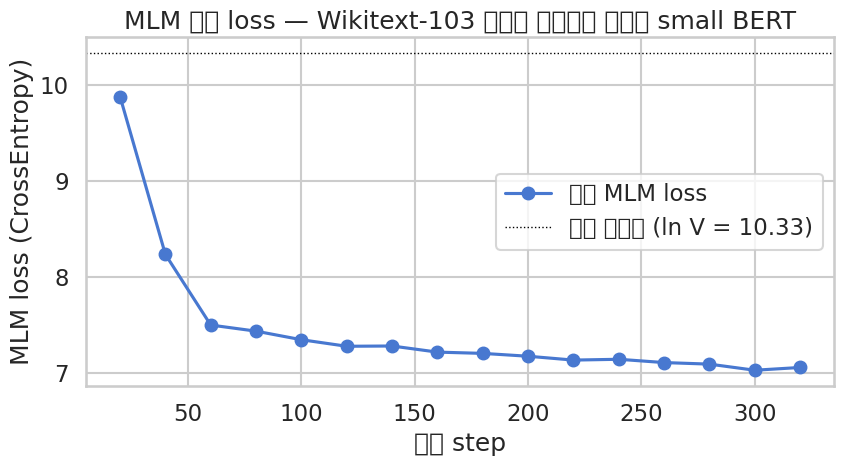
\includegraphics[width=0.82\linewidth]{assets/figures/ch20_mlm_training_loss.png}
\end{bookfigurelabel}

\textbf{그림 읽기} --- 그림~\ref{fig:ch20-mlm-training-loss}에서 다음 내용을 확인합니다: 작은 BERT의 MLM 사전학습 loss 곡선. 실행된 노트북에서 저장된 최신 plot 출력이므로, 코드에서 계산한 값이 어떤 평가 지점으로 이어지는지 바로 확인할 수 있습니다.



\Needspace{11\baselineskip}
\begin{lstlisting}
eval_metrics = trainer.evaluate()
eval_loss = eval_metrics["eval_loss"]
eval_ppl = math.exp(eval_loss)
print("=== eval (held-out Wikitext-103 paragraphs) ===")
for k, v in eval_metrics.items():
    if isinstance(v, float):
        print(f"  {k:>22}: {v:.4f}")
print()
print(f"  MLM loss:               {eval_loss:.4f}")
print(f"  perplexity (exp loss):  {eval_ppl:.2f}")
print(
    f"  random baseline PPL:    "
    f"{tokenizer.vocab_size:,}  (uniform over vocab)"
)
print(
    f"  -> model narrowed vocab to approx. "
\end{lstlisting}

\noindent\emph{앞 블록은 텍스트를 모델 입력 텐서로 바꾸는 단계입니다. 이어지는 블록에서는 앞에서 만든 중간 값을 다음 계산으로 넘기는 단계로 넘어갑니다.}

\Needspace{5\baselineskip}
\begin{lstlisting}[firstnumber=17]
    f"{eval_ppl:.0f} candidates per masked position"
)
\end{lstlisting}

\begin{codeRead}
\textbf{1행}의 \inlinecode{eval\_metrics = ...}에서는 이후 분석에서 사용할 값을 준비합니다. \textbf{2행}의 \inlinecode{eval\_loss = ...}에서는 이후 분석에서 사용할 값을 준비합니다. \textbf{3행}의 \inlinecode{eval\_ppl = ...}에서는 이후 분석에서 사용할 값을 준비합니다.
\end{codeRead}

\noindent\textbf{출력.}
\begin{bookoutputbox}
Training Loss  Validation Loss  Epoch
-------------  ---------------  -----
7.072258       7.133166         2
=== eval (held-out Wikitext-103 paragraphs) ===
               eval_loss: 7.1332

  MLM loss:               7.1332
  perplexity (exp loss):  1252.84
  random baseline PPL:    30,522  (uniform over vocab)
  -> model narrowed vocab to approx. 1253 candidates per masked position
\end{bookoutputbox}
\par\vspace{0.9em}



\subsection{사전학습 전후 비교}

학습 직전 (5번 마지막 셀에서 측정해 둔 \inlinecode{pre\_eval\_loss} / \inlinecode{pre\_top5\_records}) 와 \emph{완전히 같은 문장·같은 평가 셋} 에 학습 후 모델을 적용해 두 결과를 나란히 봅니다. \emph{사전학습이 본체에 무엇을 새겼는가} 의 가장 직접적인 증거.

\begin{quote}
학습 후 \inlinecode{eval\_loss} 는 \textbf{6 절에서 잰 값을 그대로} 씁니다. MLM 평가는 \inlinecode{DataCollatorForLanguageModeling} 이 호출할 때마다 \emph{다른 자리} 를 마스킹하므로, \inlinecode{trainer.evaluate()} 를 두 번 부르면 같은 모델·같은 평가셋인데도 값이 미세하게 달라집니다 --- 비교의 기준을 하나로 고정하기 위해 재측정하지 않습니다. 같은 이유로 \textbf{학습 로그에 찍히는 epoch 별 \inlinecode{Validation\ Loss} 도 6 절의 값과 조금씩 다릅니다} --- 오탈자가 아니라 MLM 평가가 매번 다른 자리를 마스킹하는 데서 오는 정상적인 편차입니다.
\end{quote}



\subsection{eval\_loss / perplexity --- 수치 비교}

두 측정치를 한 표·한 막대 그래프로.



\Needspace{10\baselineskip}
\begin{lstlisting}
metric_compare = pd.DataFrame({
    "metric":           ["eval_loss", "eval_perplexity"],
    "before (random)":  [pre_eval_loss,  pre_eval_ppl],
    "after (2 epoch)":  [post_eval_loss, post_eval_ppl],
    "random baseline":  [random_baseline_loss, float(tokenizer.vocab_size)],
})
print("Before vs After — eval metrics")
print(metric_compare.round(4).to_string(index=False))
\end{lstlisting}

\noindent\textbf{출력.}
\begin{bookoutputbox}
Before vs After -- eval metrics
         metric  before (random)  after (2 epoch)  random baseline
      eval_loss          10.3721           7.1332          10.3262
eval_perplexity       31955.8444        1252.8376       30522.0000
\end{bookoutputbox}
\par\vspace{0.9em}



\compactCodeOmitted{텍스트를 모델 입력 텐서로 바꾸는 단계}

\begin{bookfigurelabel}[H]{사전학습 전후 MLM eval loss와 perplexity 비교}{fig:ch20-eval-loss-ppl}
\centering
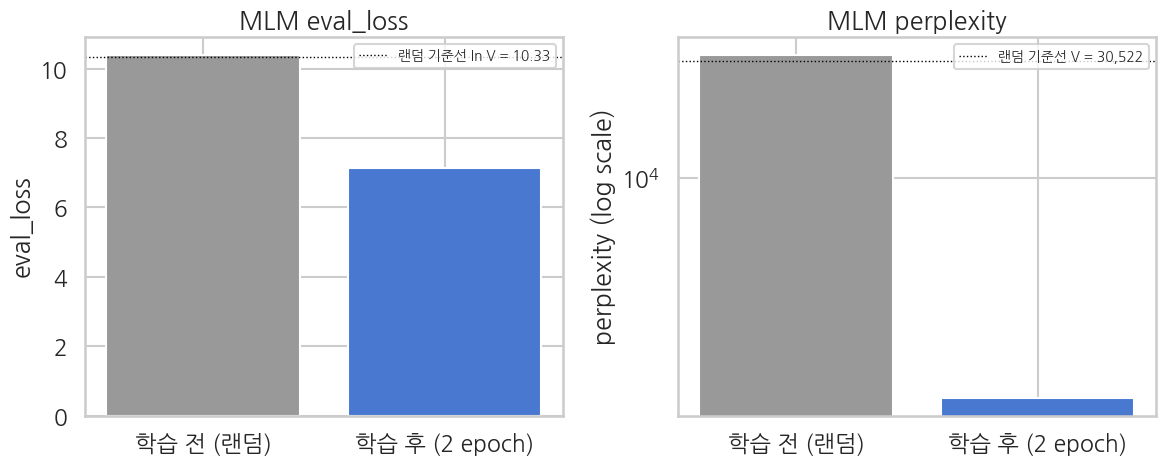
\includegraphics[width=0.88\linewidth]{assets/figures/ch20_eval_loss_ppl.png}
\end{bookfigurelabel}

\textbf{그림 읽기} --- 그림~\ref{fig:ch20-eval-loss-ppl}에서 다음 내용을 확인합니다: 사전학습 전후 MLM eval loss와 perplexity 비교. 실행된 노트북에서 저장된 최신 plot 출력이므로, 코드에서 계산한 값이 어떤 평가 지점으로 이어지는지 바로 확인할 수 있습니다.



\subsection{unigram 기준선 --- 우리 모델은 지금 무엇을 배운 상태인가}

학습 후 top-5 를 보면 \emph{어떤 문장을 넣어도 거의 같은 답} (\inlinecode{the}, \inlinecode{,}, \inlinecode{.}, \inlinecode{and} \ldots) 이 나옵니다. 버그처럼 보이지만 아닙니다 --- \textbf{문맥을 전혀 쓰지 않는 모델에게는 그게 최선의 답} 이기 때문입니다. 입력이 무엇이든 \emph{코퍼스에서 가장 흔한 토큰} 을 찍는 것이 기대 loss 를 최소화합니다.

그렇다면 “문맥은 전혀 못 쓰고 \textbf{빈도만} 아는 모델” 의 loss 는 정확히 얼마일까요? 학습 코퍼스의 \textbf{unigram 분포} 로 직접 계산해, 우리 모델이 \inlinecode{ln\ V} (균등) 와 그 사이 \emph{어디쯤} 서 있는지 확인합니다. 이 한 줄이 \emph{2 epoch 학습이 무엇을 새겼고 무엇을 아직 못 새겼는지} 를 확정해 줍니다.

\begin{quote}
엄밀히는 두 값의 측정 범위가 조금 다릅니다 --- unigram 기준선은 eval 셋 \emph{전체 토큰} 으로 계산하고, 모델의 \inlinecode{eval\_loss} 는 collator 가 고른 \emph{마스킹된 15\% 자리} 에서만 계산됩니다. 마스크 위치가 무작위 균일 표본이라 비교 자체는 타당하지만, 80/10/10 중 \emph{원본 그대로 유지되는 10\%} 에서 모델이 입력을 그대로 베껴 얻는 이득이 섞여 있어 아래 출력의 \textquotesingle 문맥으로 벌어들인 이득\textquotesingle{} 은 실제보다 조금 후하게 잡힙니다. 즉 문맥을 거의 못 배웠다는 결론은 이 보정을 감안하면 오히려 더 강해집니다.
\end{quote}



\Needspace{11\baselineskip}
\begin{lstlisting}
from collections import Counter

counter = Counter()
for ids in lm_train["input_ids"]:
    counter.update(ids)
total_tok = sum(counter.values())
V = tokenizer.vocab_size

unigram_ce = -np.mean([
    math.log((counter[i] + 1) / (total_tok + V))
    for ids in lm_eval["input_ids"] for i in ids
])
unigram_ppl = math.exp(unigram_ce)

\end{lstlisting}

\noindent\emph{앞 블록은 필요한 라이브러리와 기본 설정을 준비하는 단계입니다. 이어지는 블록에서는 앞에서 만든 중간 값을 다음 계산으로 넘기는 단계로 넘어갑니다.}

\Needspace{11\baselineskip}
\begin{lstlisting}[firstnumber=15]
print("=" * 78)
print("MLM loss 사다리 — 우리 모델은 지금 어디에 있나")
print("=" * 78)
print(
    f"  1) 균등 분포 (random init) : {random_baseline_loss:7.4f}   ppl "
    f"{V:>9,.0f}"
)
print(
    f"  2) unigram (빈도만, 문맥 X): {unigram_ce:7.4f}   ppl "
    f"{unigram_ppl:>9,.0f}"
)
print(
    f"  3) 우리 작은 BERT (2 epoch): {post_eval_loss:7.4f}   ppl "
    f"{post_eval_ppl:>9,.0f}"
)
print()
\end{lstlisting}

\noindent\emph{앞뒤 블록은 모두 앞에서 만든 중간 값을 다음 계산으로 넘기는 단계입니다. 길이를 나누어 같은 흐름을 단계별로 확인합니다.}

\Needspace{11\baselineskip}
\begin{lstlisting}[firstnumber=31]
print(
    f"  1) -> 2) : "
    f"{random_baseline_loss - unigram_ce:+.4f} nats   <- 빈도만 배워도 이만큼 내려감"
)
print(
    f"  2) vs 3) : "
    f"{unigram_ce - post_eval_loss:+.4f} nats   <- 문맥으로 벌어들인 이득 (양수면 unigram 보다 나음)"
)
print()

\end{lstlisting}

\noindent\emph{앞 블록은 앞에서 만든 중간 값을 다음 계산으로 넘기는 단계입니다. 이어지는 블록에서는 텍스트를 모델 입력 텐서로 바꾸는 단계로 넘어갑니다.}

\Needspace{11\baselineskip}
\begin{lstlisting}[firstnumber=41]
corpus_top5 = [tokenizer.convert_ids_to_tokens(i) for i, _ in counter.most_common(5)]
shared = set.intersection(*[set(r["top5_after"]) for r in post_top5_records])
shared_ordered = [t for t in post_top5_records[0]["top5_after"] if t in shared]
print(f"  학습 코퍼스 top-5 unigram : {corpus_top5}")
print(
    f"  우리 모델의 top-5         : "
    f"{post_top5_records[0]['top5_after']}"
)
print(
    f"  문장 4개가 공유하는 토큰  : {len(shared)}/5 개 — "
    f"{shared_ordered}"
)
print(
     "                              (입력이 달라져도 답이 거의 안 바뀜 = 문맥을 아직 안 읽음)"
)
\end{lstlisting}

\noindent\textbf{출력.}
\begin{bookoutputbox}
==============================================================================
MLM loss 사다리 -- 우리 모델은 지금 어디에 있나
==============================================================================
  1) 균등 분포 (random init) : 10.3262   ppl    30,522
  2) unigram (빈도만, 문맥 X):  7.2525   ppl     1,412
  3) 우리 작은 BERT (2 epoch):  7.1332   ppl     1,253

  1) -> 2) : +3.0737 nats   <- 빈도만 배워도 이만큼 내려감
2) vs 3) : +0.1193 nats <- 문맥으로 벌어들인 이득 (양수면 unigram 보다 나음)

  학습 코퍼스 top-5 unigram : ['the', ',', '.', 'of', 'and']
  우리 모델의 top-5         : ['the', ',', '.', 'and', 'in']
  문장 4개가 공유하는 토큰  : 4/5 개 -- ['the', ',', '.', 'and']
(입력이 달라져도 답이 거의 안 바뀜 = 문맥을 아직 안 읽음)
\end{bookoutputbox}
\par\vspace{0.9em}



\subsection{\texorpdfstring{표준 BERT 기준점}{표준 BERT 기준점}}

우리 작은 BERT (약 11M, 5K paragraphs \(\times\) 2 epoch) 는 방금 확인했듯 \emph{unigram 분포까지} 도달한 상태 --- 문맥은 아직 거의 못 씁니다. 이유는 단순합니다: \textbf{학습 데이터·모델 크기·학습 시간 모두 부족}. \emph{그럼 사다리의 끝, 문맥을 제대로 배운 모델은 같은 자리에 무엇을 놓나?} 를 표준 \inlinecode{bert-base-uncased} (110M, 위키+BookCorpus 약 33억 토큰) 로 직접 봅니다.

같은 토크나이저 (\inlinecode{bert-base-uncased}) 를 쓰고 있으므로 \emph{모델만 바꿔} 두 결과를 나란히.



\Needspace{11\baselineskip}
\begin{lstlisting}
def predict_mask_with(text, ref, top_k=5):
    '''임의의 MLM 모델로 [MASK] 자리 top-k 예측.'''
    ref.eval()
    inputs = tokenizer(text, return_tensors="pt").to(ref.device)
    with torch.no_grad():
        outputs = ref(**inputs)
    logits = outputs.logits[0]
    mask_positions = (inputs["input_ids"][0] == tokenizer.mask_token_id).nonzero(as_tuple=True)[0]
    if len(mask_positions) == 0:
        return None
    results = []
\end{lstlisting}

\noindent\emph{앞뒤 블록은 모두 텍스트를 모델 입력 텐서로 바꾸는 단계입니다. 길이를 나누어 같은 흐름을 단계별로 확인합니다.}

\Needspace{11\baselineskip}
\begin{lstlisting}[firstnumber=12]
    for pos in mask_positions:
        probs = torch.softmax(logits[pos], dim=-1)
        top_p, top_i = probs.topk(top_k)
        candidates = [(
            tokenizer.convert_ids_to_tokens(int(i)),
            float(p),
        )
                       for p, i in zip(top_p, top_i)]
        results.append((int(pos), candidates))
    return results

\end{lstlisting}

\noindent\emph{앞 블록은 텍스트를 모델 입력 텐서로 바꾸는 단계입니다. 이어지는 블록에서는 모델 출력을 확률이나 예측값으로 바꾸는 단계로 넘어갑니다.}

\Needspace{11\baselineskip}
\begin{lstlisting}[firstnumber=23]
ref_top5_records = []
for sent in test_sentences:
    results = predict_mask_with(sent, ref_model, top_k=5)
    top5_tokens = [tok for tok, _ in results[0][1]] if results else []
    ref_top5_records.append({"sentence": sent, "top5_ref": top5_tokens})

del ref_model
if torch.cuda.is_available():
    torch.cuda.empty_cache()
\end{lstlisting}



\subsection{{[}MASK{]} top-5 --- 3-way 비교 (before / ours / reference BERT)}

같은 문장 4개의 {[}MASK{]} 자리 top-5 후보를 \emph{사전학습 전 \(\to\) 우리 작은 BERT 학습 후 \(\to\) 표준 bert-base-uncased} 셋으로 나란히.



\textbf{해석 가이드 --- 사전학습이 만든 차이}

\begin{itemize}
\tightlist
\item
  \textbf{\inlinecode{eval\_loss}}: 균등 분포 \inlinecode{ln\ V\ ≈\ 10.33} 에서 약 7.1 까지 내려왔습니다. 다만 6-3 에서 확인했듯 그 값은 \textbf{unigram 기준선 바로 위} --- 즉 2 epoch 이 새긴 것은 대부분 \emph{“어떤 토큰이 흔한가”} 라는 \textbf{빈도 통계} 이고, \emph{“앞뒤 문맥상 무엇이 와야 하는가”} 는 아직 거의 못 배웠습니다.
\item
  \textbf{\inlinecode{perplexity}}: 30,522 (vocab 전체) 에서 약 1,250 부근으로. \emph{마스크 자리마다 후보를 약 1,250 개로 좁힌 상태} 라는 직관적 해석. 이 역시 unigram 모델이 도달하는 수준과 거의 같습니다.
\item
  \textbf{top-5 토큰} (3-way 비교):

  \begin{itemize}
  \tightlist
  \item
    \emph{before (random)}: \textbf{빈도 순위와도 문맥과도 무관한 난수 토큰} --- 조각 토큰 (\inlinecode{\#\#…})이나 희귀어가 섞이기도 하고, 평범한 중간 빈도 단어가 나오기도 합니다 (\inlinecode{SEED} 를 바꾸면 달라집니다). logits 가 순수한 난수라 \emph{어떤 토큰도 특별히 유리하지 않습니다}.
  \item
    \emph{ours (small BERT, 5K paragraphs \(\times\) 2 epoch)}: 입력 문장이 무엇이든 \textbf{거의 똑같은 top-5} (\inlinecode{the}, \inlinecode{,}, \inlinecode{.}, \inlinecode{and} \ldots) --- 6-3 에서 계산한 \emph{코퍼스 최상위 unigram 과 사실상 같은 목록} 입니다. 끝자리가 \inlinecode{of}/\inlinecode{in} 처럼 \textbf{빈도가 엇비슷한 토큰 사이에서만 흔들릴 뿐}, 입력이 바뀌어도 답이 사실상 그대로라는 것은 \textbf{모델이 아직 문맥을 읽지 않는다} 는 뜻입니다. 실패가 아니라 \emph{MLM 학습이 반드시 거치는 첫 계단} --- 문맥을 배우기 전에 주변 분포부터 배웁니다.
  \item
    \emph{ref (bert-base-uncased, 약 33억 토큰 \(\times\) 40 epoch)}: 입력마다 \textbf{답이 달라집니다} --- \texttt{The\ capital\ of\ France\ is\ {[}MASK{]}} 에는 \inlinecode{paris}, \inlinecode{lille}, \inlinecode{lyon} 처럼 \emph{프랑스 도시} 가, Yelp 문장에는 \inlinecode{delicious}, \inlinecode{amazing}, \inlinecode{highly} 같은 \emph{감성 표현} 이 옵니다. \textbf{문맥을 읽는다는 것의 관찰 가능한 증거} 가 바로 이 “입력이 바뀌면 답도 바뀐다” 입니다.
  \end{itemize}
\end{itemize}

\begin{quote}
주의 \textbf{ref 의 답이 곧 \textquotesingle 정답\textquotesingle{} 은 아닙니다.} \texttt{Water\ freezes\ at\ {[}MASK{]}\ degrees\ Celsius.} 에 \inlinecode{bert-base-uncased} 는 \inlinecode{100}, \inlinecode{60}, \inlinecode{50} \ldots{} 을 내놓습니다 --- 물이 어는 온도는 0 인데 말이죠. MLM 이 배우는 것은 \emph{세상의 사실} 이 아니라 \textbf{“이 자리에 올 법한 토큰의 분포”} 입니다. 위키 문서에서 \inlinecode{...\ degrees\ Celsius} 앞에 가장 자주 오는 숫자가 \inlinecode{100} 이기 때문에 그렇게 답하는 것. 사전학습 모델을 \emph{지식 베이스} 로 착각하면 안 되는 이유이고, 그래서 downstream task 마다 \textbf{fine-tune} 이 필요합니다.
\end{quote}

\begin{quote}
\textbf{세 모델의 격차 = 데이터 규모 + 모델 크기 + 학습 시간의 격차} --- 우리 작은 BERT (약 11M, 5K paragraphs, 2 epoch) \(\to\) reference (110M, 3.3B tokens, 40 epoch) 사이에 \emph{데이터 약 5,000배, 파라미터 약 10배, epoch 20배}. 그 격차가 “빈도만 아는 단계” 와 “문맥을 읽는 단계” 의 질적 차이로 드러납니다.
\end{quote}

이 장의 작은 BERT 는 \emph{Wikitext-103 5K paragraphs \(\times\) 2 epoch} 로 학습한 \emph{일반 도메인 mini BERT} --- \textbf{빈도 통계까지 새겨진 본체} 입니다. \ref{ch:21}장에서 Yelp 이진 분류로 fine-tune 하며 \emph{그 정도 본체라도 random init 보다 나은가} 를 직접 측정합니다 --- \emph{우리가 직접 만든 작은 영어 BERT (일반 위키 5K, 약 11M)} vs \emph{\ref{ch:10}장의 DistilBERT (대규모 Wikipedia+BookCorpus, 약 66M)} vs \emph{random init baseline}.



\section{모델 저장 --- \ref{ch:21}장에서 재사용}

\inlinecode{model.save\_pretrained()} 와 \inlinecode{tokenizer.save\_pretrained()} 를 \emph{같은 폴더} 에 저장. \ref{ch:21}장에서는 \inlinecode{AutoModelForSequenceClassification.from\_pretrained("./ch20\_small\_bert\_mlm",\ num\_labels=2)} 한 줄로 \emph{이 BERT body} 를 가져와 분류 헤드를 새로 얹습니다.



\Needspace{11\baselineskip}
\begin{lstlisting}
SAVE_DIR = "./ch20_small_bert_mlm"
model.save_pretrained(SAVE_DIR)
tokenizer.save_pretrained(SAVE_DIR)

import os
print(f"Saved to: {SAVE_DIR}")
print(f"Files:")
for f in sorted(os.listdir(SAVE_DIR)):
    size = os.path.getsize(os.path.join(SAVE_DIR, f))
    if size > 1024 * 1024:
        size_str = f"{size / 1024 / 1024:.1f} MB"
    else:
        size_str = f"{size / 1024:.1f} KB"
    print(f"  {f:>30s}  {size_str}")
\end{lstlisting}



\textbf{저장된 파일 구조} --- \inlinecode{from\_pretrained} 가 인식하는 HF 표준 레이아웃:

\begin{booktable}{20장 모델 저장 - 21장에서 재사용 표}{tab:ch20-07}
\begin{adjustbox}{max width=\textwidth}
\begin{tabular}{@{}ll@{}}
\toprule
파일 & 역할 \\
\midrule

\inlinecode{config.json} & \inlinecode{BertConfig} 직렬화 (hidden, layer, head, vocab 등) \\
\inlinecode{model.safetensors} (또는 \inlinecode{pytorch\_model.bin}) & 모델 weight \\
\inlinecode{tokenizer.json} / \inlinecode{vocab.txt} & 토크나이저 (\ref{ch:21}장 fine-tune 에서 같은 토크나이저 사용) \\
\inlinecode{special\_tokens\_map.json}, \inlinecode{tokenizer\_config.json} & 특수 토큰 메타 \\
\bottomrule
\end{tabular}
\end{adjustbox}
\end{booktable}

\begin{quote}
\ref{ch:21}장에서 \inlinecode{AutoModelForSequenceClassification.from\_pretrained("./ch20\_small\_bert\_mlm",\ num\_labels=2)} 호출 시, \inlinecode{BertForMaskedLM} 의 \emph{MLM head 는 버려지고} encoder body 만 가져옴. 그 위에 새 \inlinecode{Linear(256,\ 2)} 분류 헤드를 random init 으로 부착 --- \ref{ch:07}--\ref{ch:18}장의 fine-tune 셋업과 \emph{동일한 구조}. 이 장의 사전학습이 \emph{얼마나 도움 됐는지} 가 \ref{ch:21}장의 학습 곡선에서 직접 비교됩니다.
\end{quote}



\section{변형: 학습 step 더 늘리거나 block\_size 변경}

작은 BERT 의 성능은 \emph{학습량} 에 민감합니다. 두 가지 변형을 시뮬레이션 (실제 실행은 시간 관계상 한 셋업만):

\begin{booktable}{20장 변형: 학습 step 더 늘리거나 block\_size 변경 표}{tab:ch20-08}
\begin{adjustbox}{max width=\textwidth}
\begin{tabular}{@{}llll@{}}
\toprule
변형 축 & 이 장 (기본) & 변형 예 & 예상 효과 \\
\midrule

\inlinecode{num\_train\_epochs} & 2 & 5 & eval loss 소폭 하락 --- 부록 실측으로 ppl 1,173 \(\to\) 928 (약 20\% 감소, epoch 4 부터 평탄) \\
\inlinecode{BLOCK\_SIZE} & 128 & 64 & 블록 수 약 2배, 한 블록 짧아져 \emph{문맥} 줄음 \(\to\) loss 약간 상승 \\
\inlinecode{BLOCK\_SIZE} & 128 & 256 & 블록 수 절반, 한 블록 길어 \emph{문맥} 풍부 \(\to\) loss 하락 가능, VRAM 약 4배 (attention \(O(n^2)\)) \\
\inlinecode{N\_TRAIN\_TEXT} & 5,000 paragraphs & 30,000 paragraphs & loss 큰 폭 하락, 학습 step 약 6배 (본편 2 epoch 이 336 step / 20-25초이므로 약 2 분) --- 30분 룰 안에서 2 epoch 이상 여유 \\
\inlinecode{mlm\_probability} & 0.15 & 0.30 & 더 어려운 task \(\to\) loss 상승, 학습 신호 증가 (논문 BERT 는 15\% 가 sweet spot) \\
\bottomrule
\end{tabular}
\end{adjustbox}
\end{booktable}

\begin{quote}
\textbf{T4 30분 룰 안에서 가능한 가장 큰 개선} --- 본편은 batch 32 기준 한 epoch 이 \textbf{167 step}, 2 epoch 336 step 이 \textbf{20-25초} (준비 포함 0.4분) 로 끝납니다. 같은 batch 로 5K \(\to\) 20K (약 4배) 로 늘려도 한 epoch 은 668 step \(\approx\) \textbf{1분 안팎}. 즉 30분 룰의 병목은 학습 step 이 아니라 \textbf{데이터 준비} (다운로드·토크나이즈·\inlinecode{group\_texts}) 쪽이니, 그쪽에 여유를 크게 잡고 \emph{epoch 보다 데이터} 를 늘리는 편이 이득입니다. 이 장의 \emph{짧고 빠른} 실험 이후 직접 변형해 보세요.
\end{quote}



\subsection{사전학습을 더 돌리면? --- 부록 곡선 (이슈 \#19)}

본편은 \textbf{2 epoch} 데모라 perplexity 가 높습니다. 부록 \inlinecode{20\_en\_bert\_pretrain\_scaling} 에서 2 \(\to\) 16 epoch 으로 길게 학습하며 측정한 곡선을 보면, perplexity 가 \textbf{영어 1,173 \(\to\) 697, 한국어 1,626 \(\to\) 707 로 \textasciitilde2배} 내려간 뒤 \textbf{epoch 8-10 부터 평탄} 해집니다. (부록의 2 epoch 값 1,173 은 본편 실행본의 1,253 보다 낮습니다 --- 모델도 데이터도 같은데 \textbf{학습률 스케줄의 총 길이가 다르기} 때문입니다. 본편은 2 epoch 에 맞춰 linear decay 가 끝나도록 잡혀 후반부엔 학습률이 거의 0 인 반면, 부록은 16 epoch 짜리 스케줄이라 같은 \emph{2 epoch 지점} 에서는 아직 높은 학습률로 달리는 중입니다. 같은 “2 epoch” 라도 그때까지 겪은 학습률 경로가 다른 것.) 5,000 텍스트로는 모델이 금세 saturate 해 \emph{epoch 만으로는 한계} --- 더 낮추려면 \textbf{데이터 양} 을 늘려야 합니다 (\ref{ch:21}장 부록의 \textquotesingle 데이터가 가장 큰 lever\textquotesingle{} 와 같은 결론). 본편의 높은 perplexity 는 버그가 아니라 \emph{짧은 데모 학습의 정직한 반영} 입니다.



\section{이 장에 등장한 라이브러리·함수}

\begin{booktable}{20장 새로 등장한 라이브러리}{tab:ch20-09}
\begin{adjustbox}{max width=\textwidth}
\begin{tabular}{@{}lll@{}}
\toprule
이름 & 한 줄 설명 & 다음 장에서 \\
\midrule

\inlinecode{transformers.BertConfig} & BERT 구조 hyperparam 컨테이너 (hidden, layer, head 등) & \ref{ch:22}장에서 한국어 작은 BERT 설계 \\
\inlinecode{transformers.BertForMaskedLM} & encoder + MLM head, MLM 사전학습 전용 모델 클래스 & \ref{ch:22}장에서 한국어 MLM \\
\inlinecode{transformers.DataCollatorForLanguageModeling} & 매 batch 마다 자동 masking (15\% rule) & \ref{ch:22}장 같음 \\
\inlinecode{BertForMaskedLM(config)} (random init) & pretrained weight 없이 모델 생성 & \ref{ch:22}장 같음 \\
\inlinecode{load\_dataset("Salesforce/wikitext",\ "wikitext-103-raw-v1")} & Wikitext-103 HF 정제본 로드 (line 단위) & \ref{ch:22}장 한국어 Wikipedia (\inlinecode{wikimedia/wikipedia}) 와 같은 패턴 \\
\inlinecode{group\_texts} 패턴 (HF run\_mlm.py 표준) & 가변 길이 텍스트를 고정 길이 블록 스트림으로 & \ref{ch:22}장 같음 \\
\inlinecode{model.save\_pretrained()} / \inlinecode{from\_pretrained()} & HF 표준 체크포인트 인터페이스 & \ref{ch:21}장에서 분류 fine-tune 로드 \\
\inlinecode{math.log(vocab\_size)} & MLM 의 random baseline loss & 사전학습 장 공통 진단 도구 \\
\bottomrule
\end{tabular}
\end{adjustbox}
\end{booktable}



\section{체크포인트 질문}

\begin{enumerate}
\def\labelenumi{\arabic{enumi}.}
\tightlist
\item
  MLM 사전학습의 random baseline loss 가 \inlinecode{ln(30522)\ ≈\ 10.33} 인 이유는 무엇이고, 학습 첫 step 의 loss 가 이 값과 \emph{크게} 다르다면 무엇을 의심해야 하나요? 또 학습 후 loss 가 \textbf{unigram 기준선 근처에서 멈춰 있다면} 모델은 무엇을 배웠고 무엇을 아직 못 배운 상태인가요?
\item
  \inlinecode{DataCollatorForLanguageModeling} 이 매 batch 마다 \emph{다른} 위치를 mask 합니다. 같은 위치를 \emph{고정해서} mask 하면 어떤 문제가 생길까요?
\item
  \inlinecode{BertForMaskedLM} 의 MLM head 가 \emph{입력 임베딩과 tied} 됩니다. 왜 이렇게 묶으면 파라미터 절약 + 학습 안정에 모두 도움이 되나요?
\item
  \ref{ch:21}장에서 \inlinecode{AutoModelForSequenceClassification.from\_pretrained("./ch20\_small\_bert\_mlm",\ num\_labels=2)} 를 호출하면, \emph{이 장 모델의 어떤 부분} 이 이어지고 \emph{어떤 부분} 이 버려지나요?
\end{enumerate}



\section{FAQ}

\begin{faqBox}{Q1. (이론) 왜 Yelp text 가 아니라 일반 위키 (Wikitext-103) 로 사전학습하나요? \ref{ch:21}장의 분류가 Yelp 인데 같은 도메인으로 학습하는 게 더 유리하지 않나요?}

\textbf{일반 도메인 \(\to\) 다른 도메인 transfer} 가 \emph{진짜 사전학습-fine-tune 패러다임} 이기 때문입니다. Yelp text 로 MLM 사전학습 \(\to\) Yelp 분류 fine-tune 의 흐름은 사실 \emph{domain-adaptive pretraining} (DAPT) 에 더 가깝습니다 --- 사전학습이 \emph{이미 task 도메인의 표현} 을 학습한 상태에서 분류만 얹는 셈.

원본 BERT (Devlin et al., 2018) 가 \emph{Wikipedia + BookCorpus} 라는 일반 도메인 코퍼스로 사전학습한 뒤 \emph{완전히 다른} GLUE/SQuAD task 로 fine-tune 한 게 \emph{transfer 의 본질} --- 일반 표상이 다른 도메인에도 적용 가능한가의 시험.

\Needspace{5\baselineskip}
\begin{lstlisting}

\end{lstlisting}

\ref{ch:22}--\ref{ch:23}장의 한국어 흐름 (한국어 Wikipedia \(\to\) NSMC 영화 리뷰) 도 \emph{대칭} 패턴. 일반 위키 학습이 task 도메인 fine-tune 에 \emph{얼마나 효율적으로 transfer 되는가} 가 본 장의 진짜 측정 대상.

\begin{quote}
\textbf{참고} --- \ref{ch:10}장 (DistilBERT) 도 Wikipedia + BookCorpus 사전학습 \(\to\) Yelp 분류 fine-tune 의 \emph{같은 패턴}. 본 장의 작은 BERT 와 \ref{ch:10}장의 DistilBERT 가 \emph{같은 일반 도메인 사전학습 \(\to\) 같은 task fine-tune} 이라 \emph{공정한 비교} 가 됩니다. Yelp 로 사전학습했다면 \ref{ch:10}장과 비교 자체가 unfair.
\end{quote}

\end{faqBox}


\begin{faqBox}{Q3. (이론) \inlinecode{mlm\_probability=0.15} 의 15\% 는 어디서 나온 숫자인가요?}

BERT 원논문 (Devlin et al., 2018, arXiv:1810.04805) 의 sweet spot:

\begin{itemize}
\tightlist
\item
  너무 작으면 (5\% 정도): 한 batch 의 \emph{학습 신호} (loss 가 계산되는 위치) 가 너무 적어 학습 효율 \(\downarrow\)
\item
  너무 크면 (40\%+): 모델이 \emph{문맥} 으로 볼 수 있는 토큰이 너무 적어 mask 추측이 \emph{불가능에 가까워짐}. loss 가 크지만 학습 가치는 작음
\item
  15\% 가 \emph{학습 신호 양 + 추측 가능성} 의 균형점
\end{itemize}

후속 연구 (RoBERTa, ELECTRA) 는 \emph{동적 masking} (매 batch 다른 위치, 이미 본 장에서 collator 가 자동 처리) 또는 \emph{교체-기반 학습} (ELECTRA) 같은 변형을 시도했지만, \emph{15\% mask 비율} 자체는 거의 표준으로 정착.

\end{faqBox}


\begin{faqBox}{Q5. (실무) 사전학습이 \emph{얼마나} 도움 되는지 어떻게 확인하나요?}

\ref{ch:21}장에서 두 모델을 \emph{같은 분류 task} 로 fine-tune 해 비교하는 게 가장 직접적입니다:

\Needspace{11\baselineskip}
\begin{lstlisting}
model_pretrained = AutoModelForSequenceClassification.from_pretrained(
    "./ch20_small_bert_mlm", num_labels=2
)

config = BertConfig(
    hidden_size=256,
    num_hidden_layers=4,
    ...,
)
model_scratch = BertForSequenceClassification(config)
\end{lstlisting}

두 모델을 \emph{같은 Yelp 이진 학습 데이터} 로 fine-tune \(\to\) eval accuracy 비교. 사전학습이 도움 됐다면 (A) 가 (B) 보다 \emph{빨리} 그리고 \emph{높이} 도달. \ref{ch:21}장의 핵심 실험.

\begin{quote}
\textbf{참고}: 이 장의 \emph{작은 사전학습} (5K 문장, 1-2 epoch) 은 \emph{큰 효과} 를 기대하기 어렵습니다. 그러나 \emph{방향성} (random 보다 시작점이 낫다) 은 분명히 나옵니다. 큰 효과를 보려면 데이터 100K+, epoch 5+, BERT 표준 크기 --- 이건 T4 30분 룰 밖.
\end{quote}

\end{faqBox}






\compactFAQMore{5}

\begin{previewBox}{미리보기: 다음 장}

\textbf{\ref{ch:21}장. 영어 BERT 분류 (\ref{ch:20}장 사전학습 모델 fine-tune) --- \emph{일반 도메인 \(\to\) 다른 도메인 transfer}}

\begin{itemize}
\tightlist
\item
  이 장의 \inlinecode{./ch20\_small\_bert\_mlm} 체크포인트를 \inlinecode{AutoModelForSequenceClassification.from\_pretrained(...,\ num\_labels=2)} 로 로드 \(\to\) MLM head 떼고 분류 헤드 부착
\item
  \textbf{Yelp 이진 분류 fine-tune} (\ref{ch:10}·\ref{ch:11}장과 같은 데이터·셋업) --- \emph{완전히 다른 도메인 transfer}. 일반 위키로 사전학습한 본체가 \emph{Yelp 리뷰(식당·업체) 도메인} 에 얼마나 잘 적응하는가 측정
\item
  \textbf{핵심 비교}: 이번 작은 사전학습 BERT (약 11M params, Wikitext-103 5K paragraphs MLM) vs \ref{ch:10}장의 DistilBERT (약 66M params, 대규모 Wikipedia + BookCorpus 사전학습). 둘 다 \emph{일반 도메인 \(\to\) Yelp transfer} 라 비교가 \emph{fair} --- \emph{사전학습 규모} 차이만 측정됨
\item
  작은 모델 + 작은 데이터 사전학습이 \emph{얼마나 도움 되는가} 의 정량 측정 --- fine-tune 학습 곡선·최종 accuracy·confusion matrix 모두 나란히
\item
  일부러 \emph{random init} baseline (사전학습 없이 분류 직접) 도 함께 학습해 \emph{사전학습의 순 효과} 분리
\end{itemize}

\begin{quote}
\textbf{변하는 축}: Phase 3 안에서 \emph{task 가 사전학습 (MLM) \(\to\) 분류 (fine-tune)} 로 전환. 모델 구조·토크나이저는 그대로, 데이터 도메인이 \emph{위키 \(\to\) Yelp} 로 바뀌고 loss·평가 metric 이 분류 표준으로 돌아옴.
\end{quote}
\end{previewBox}



\Needspace{18\baselineskip}

\section{온라인 부록: 사전학습량과 perplexity}

\onlineAppendixLink{사전학습량과 perplexity}{영어 perplexity는 1,173에서 697로, 한국어는 1,626에서 707로 내려가지만 8--10 epoch 이후에는 개선이 평탄해집니다. 같은 5,000개 텍스트를 반복하는 것보다 데이터와 compute를 늘리는 편이 다음 성능 레버라는 결론입니다.}{https://colab.research.google.com/github/yoon-gu/neuqes-101/blob/master/20_en_bert_pretrain/20_en_bert_pretrain_scaling.ipynb}

\begin{bookfigurelabel}[H]{사전학습 epoch에 따른 영어와 한국어 MLM perplexity}{fig:ch20-pretrain-scaling-curve}
\centering
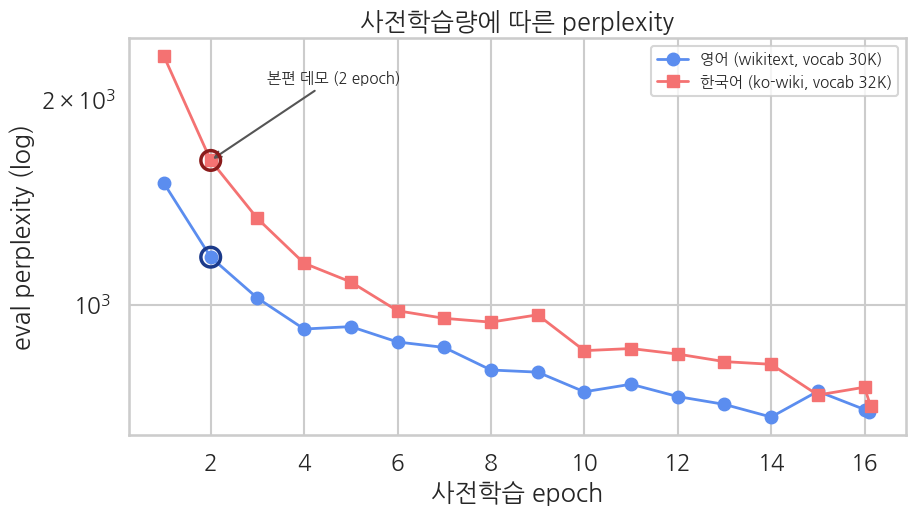
\includegraphics[width=0.72\linewidth]{assets/figures/ch20_pretrain_scaling_curve.png}
\end{bookfigurelabel}

\textbf{그림 읽기} --- 그림~\ref{fig:ch20-pretrain-scaling-curve}에서 다음 내용을 확인합니다: 사전학습 epoch에 따른 영어와 한국어 MLM perplexity. 실행된 노트북에서 저장된 최신 plot 출력이므로, 코드에서 계산한 값이 어떤 평가 지점으로 이어지는지 바로 확인할 수 있습니다.